\documentclass[tikz]{standalone}
\usepackage{calc}
\begin{document}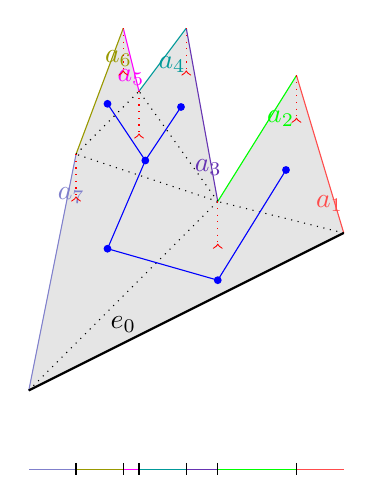
\begin{tikzpicture}[scale=2]
\coordinate (x0) at (0,0);
\coordinate (x1) at (2,1);
\coordinate (x2) at (1.7,2);
\coordinate (x3) at (1.2,1.2);
\coordinate (x4) at (1,2.3);
\coordinate (x5) at (.7,1.9);
\coordinate (x6) at (.6,2.3);
\coordinate (x7) at (.3,1.5);

\coordinate (xb0) at (0,0);
\coordinate (xb1) at (2,0);
\coordinate (xb2) at (1.7,0);
\coordinate (xb3) at (1.2,0);
\coordinate (xb4) at (1,0);
\coordinate (xb5) at (.7,0);
\coordinate (xb6) at (.6,0);
\coordinate (xb7) at (.3,0);

\coordinate (t0) at (barycentric cs:x0=2,x1=3,x3=1);
\coordinate (t1) at (barycentric cs:x1=1,x2=1,x3=1);
\coordinate (t2) at (barycentric cs:x0=1,x3=1,x7=1);
\coordinate (t3) at (barycentric cs:x3=2,x5=1,x7=2);
\coordinate (t4) at (barycentric cs:x3=1,x4=1,x5=1);
\coordinate (t5) at (barycentric cs:x4=1,x6=1,x7=3);

\definecolor{cola}{rgb}{1,.3,.3};
\definecolor{colb}{rgb}{0,1,0};
\definecolor{colc}{rgb}{0.4,0.2,.7};
\definecolor{cold}{rgb}{0,.6,.6};
\definecolor{cole}{rgb}{1,0,1};
\definecolor{colf}{rgb}{.6,.6,0}
\definecolor{colg}{rgb}{.5,.5,.8};

\fill[fill=gray!20] (x0) -- (x1) -- (x2) -- (x3) -- (x4) -- (x5) -- (x6) -- (x7) -- (x0) -- cycle;
\draw[cola] (x1) -- node[pos=0.3,below] {$a_1$} (x2);
\draw[colb] (x2) -- node[pos=0.2,below] {$a_2$} (x3);
\draw[colc] (x3) -- node[pos=0.3,below] {$a_3$} (x4);
\draw[cold] (x4) -- node[pos=0.3,below] {$a_4$} (x5);
\draw[cole] (x5) -- node[pos=0.5,below] {$a_5$} (x6);
\draw[colf] (x6) -- node[pos=0.1,below] {$a_6$} (x7);
\draw[colg] (x7) -- node[pos=0.1,below] {$a_7$} (x0);

\draw[cola] (0,-.5) +(xb1) -- +(xb2);
\draw[colb] (0,-.5) +(xb2) -- +(xb3);
\draw[colc] (0,-.5) +(xb3) -- +(xb4);
\draw[cold] (0,-.5) +(xb4) -- +(xb5);
\draw[cole] (0,-.5) +(xb5) -- +(xb6);
\draw[colf] (0,-.5) +(xb6) -- +(xb7);
\draw[colg] (0,-.5) +(xb7) -- +(xb0);

\foreach \i in {2,3,...,7}
 \draw (xb\i) +(0,-.46) -- +(0,-.54);

\draw[thick] (x0) -- node[pos=0.3,above] {$e_0$} (x1);
\draw[dotted] (x0) -- (x3);
\draw[dotted] (x1) -- (x3);
\draw[dotted] (x3) -- (x7);
\draw[dotted] (x3) -- (x5);
\draw[dotted] (x7) -- (x5);

\foreach \i in {2,3,4,5,6,7}
\draw[red,-<,dotted] (x\i) -- +(0,-.3);

\foreach \i in {0,1,2,3,4,5}
\node[circle,fill,blue,inner sep=1pt] at (t\i) {};

\draw[blue] (t0) -- (t1);
\draw[blue] (t0) -- (t2) -- (t3) -- (t4);
\draw[blue] (t3) -- (t5);


\end{tikzpicture}\end{document}
